%!TEX root = P231_2023.tex


This is a \emph{crash course} in the mathematical toolkit necessary for graduate courses in electrodynamics, quantum mechanics, and statistical mechanics. The emphasis is physical intuition rather than mathematical rigor. Let us be clear: as a student you are \emph{expected} to be as mathematically rigorous as your specific discipline requires. Fortunately, there are plenty of excellent textbooks targeted at various levels of rigor and you can find the one most appropriate for you. This course is meant to complement those references, not to replace them.\footnote{In other words, this is \emph{your} \acro{Ph.D}, craft it appropriately.}

\emph{Unfortunately}, the choice of topics in this course will be neither necessary nor sufficient for your training. If anyone asks, you should say that the theme of this course is to solve the types of linear differential equations that will show up in your physics coursework (\emph{ugh! Boring!}). The actual choice of topics is meant to highlight larger, unifying themes in mathematical physics sprinkled with topics of current research significance.


\section{Green's functions and this course}

Our goal is to solve linear differential equations:
\begin{align}
  \mathcal O f(x) = s(x) \ .
  \label{eq:greens:function:equation}
\end{align}
In this equation, $\mathcal O$ is a \emph{differential operator}\index{differential operator} that encodes some kind of physical dynamics\footnote{A \textbf{differential operator} is just something built out of derivatives that can act on a function. The differential operator may contain coefficients that depend on the variable that we are differentiating with respect to; for example, $\mathcal O = (d/dx)^2 + 3x\,(d/dx)$.}, $s(x)$ is the \emph{source} of those dynamics, and $f(x)$ is the system's physical \emph{response} that we would like to determine. The solution to this equation is:
\begin{align}
  f(x) &= \mathcal O^{-1} s(x) \ .
\end{align}
This statement is trivial and deeply unsatisfying. We will think carefully about what $\mathcal O^{-1}$ actually means and how to calculate it. $\mathcal O^{-1}$ is the \textbf{Green's function}\index{Green's function} for the differential operator $\mathcal O$. 

\begin{exercise}%
Consider the differential operator $\mathcal O = (d/dx)^2 + 3x\,(d/dx)$. A colleague tells you that $(d/dx)^2$ is squared, therefore it is not a linear operator. Explain why the colleague is mistaken. 
\end{exercise}

To make sense of the object $\mathcal O^{-1}$, we appeal to linear algebra. A linear transformation---that is, a \textbf{matrix}---$A$ acts on a vector $\vec{v}$ to give equations like
\begin{align}
  A \vec{v} = \vec{w} \ ,
\end{align}
whose solution is
\begin{align}
  \vec{v} = A^{-1} \vec{w} \ .
\end{align}
In this course, we think of linear differential operators $\mathcal O$ as infinite-dimensional matrices. $\mathcal O^{-1}$ is the inverse of this matrix. Perhaps you feel a bit nervous because you remember that inverse of a $3\times 3$ matrix is tricky... say nothing of the \emph{infinite} dimensional limit. To assuage this doubt, we remind ourselves that that calculus is infinite-dimensional linear algebra. Complex analysis extends the real line to the complex plane. In so doing, the \emph{analytic structure} of our theories offer both a method to calculate challenging integrals and their own physical significance. 

% In order to guide our studies, we shall have one primary example in the back of our mind:  the humble harmonic oscillator. In subsequent chapters we extend this to higher-dimensions and, indeed, to \emph{infinite} dimensions. Along the way we reflect on the nature of all of these infinities we bandy about. We close by connecting our study of Green's functions to statistics, non-perturbative methods, and the burgeoning connections of physics to machine learning.

% In your graduate studies, you will find yourself becoming intimately familiar with a bestiary of Bessel functions, Hankel functions, Legendre polynomials and spherical harmonics. These are special functions that show up in common models of physical systems. In a perverse parallel universe, this course would pummel you with the properties of these functions. However, in an era where manipulating these functions becomes a trivial exercise with \emph{Mathematica}\footnote{Or the open source alternative of your choice. Perhaps simply asking \emph{Wolfram Alpha} or \acro{ChatGPT}.}, the the key to a physics education is to understand how these sophisticated functions are simply cousins of humbler sines and cosines.



\section{This is not what I expected}


This is a course in mathematical methods for \emph{physicists}.
%
We do not solve \emph{every} class of differential equation that is likely to pop up in your research careers---that would be a course on mathematical methods for \emph{engineers}.\footnote{I recommend Carl Bender's 2011 lectures at \acro{PSI} for an insightful course along those lines~\cite{pirsa_11110040}.} Instead, we methodically dissect a physically motivated example---the harmonic oscillator---to emphasize how we think about mathematical problems. 

We weave together ideas that are not often connected explicitly in undergraduate physics courses: linear algebra, differential equations, complex analysis, statistics. I expect that you have had some formal training in these topics so that we may focus on the \emph{interconnections} between these ideas in our study of nature.

Do not be surprised if we only mention Bessel functions in passing. Do not think less of our efforts if we do not calculate Wronksians or go beyond a single Riemann sheet. As graduate students, it is \emph{your} responsibility to be able to grab your favorite reference to apply mathematics as needed to \emph{your} research. \emph{This} course is about the larger narrative that is not often shared explicitly in those books. It is about that which makes physicists employable in Silicon Valley while simultaneously terrible at splitting the bill at a restaurant. 

\begin{example}
Our cavalier attitude towards mathematical rigor should not make you think that mathematical rigor is not necessary. For a nice, visual example, see ``How to lie using visual proofs'' by 3Blue1Brown.\cite{3Blue1Brown_2022}
% https://youtu.be/VYQVlVoWoPY
\end{example}



\section{The non-mathematical idea of niceness}
\label{sec:niceness}

I find it useful to invoke the notion of a \textbf{nice}\index{nice} mathematical situation. This is not a formal idea. In fact, it is one of many things that mathematicians find ridiculous about me. However, as a physicist, the concept of mathematical \emph{niceness} is remarkably helpful.

The physical systems that we spend the most time thinking about are all \emph{nice}. 
%
While mathematicians spend years proving every exceptional case to a theorem, we are happy to push onward as long as our mathematical results are true for the \emph{nice} cases. 
%
In fact, nature often admits an \emph{approximately} nice mathematical description.\footnote{This is not because nature is kind, but rather because we are only clever enough to build simple theories. What is important to appreciate as a physicist is \emph{why} simple theories can so nearly approximate nature.}

%
Nice mathematical models make tidy predictions. Then we can Taylor expand about these nice predictions to make better predictions.
%
We sometimes chant \emph{perturbation theory}\index{perturbation theory} out loud several times in case someone watching us does not think we are being rigorous enough.\footnote{Sometimes our Taylor expansions have zero radius of convergence. ``\emph{E pur si muove},'' as Galileo would say. Look up the convergence of the Dyson series.}
% We make Taylor expansions without anguishing about the radius of convergence\footnote{\url{https://johncarlosbaez.wordpress.com/2016/09/21/struggles-with-the-continuum-part-6/}} and validate it post-facto because it \emph{works}.


This is not to say that nature cares at all about our simple physical models. 
%
Every once in a while, we \emph{do} have to worry about the exceptional cases because our models fail to accommodate what is \emph{actually} happening in nature.\footnote{Full disclosure: Your \acro{Ph.D} will likely depend on finding a clever solution to one of these cases.} Those scenarios are the most exciting of all: that is when our mathematical formalism grabs us by the collar and says, \emph{listen to me---something important is happening!} This often happens when a calculation tells us that a physical result is infinite. 

\begin{exercise}\label{ex:hydrogen:problem}
Consider the potential that an electron feels in the hydrogen atom:
\begin{align}
  V(r) &= -\frac{\alpha}{r} \ .
\end{align}
As the electron--proton separation goes to zero, $r\to 0$, the potential goes to infinity. Classical electrodynamics is telling us that something curious is happening. What actually happens? (And why didn't you ask this question when you were in high school?)
\end{exercise}

We focus on \emph{nice} functions and \emph{nice} operators and \emph{nice} boundary conditions, and so forth. We often only need the \emph{nice} math to make progress on our \emph{nice} physical models. It is worth spending our time learning to work with these \emph{nice} limits. Leave the degenerate cases to the mathematicians for now. Eventually, you will find yourself in a situation where physics demands \emph{not nice} mathematics. In that case---and only when the physics demands it---you will be ready to poke and prod at the mathematical curiosity until the underlying \emph{physics} reason for the not-niceness is apparent. All this is to say: if you object to this course because we do not start with proofs about open sets or convergence, then you are missing the point of an education in physics.




\section{The unbearable arrogance of physicists}
\label{sec:obvious}

Sometimes physicists have a reputation for arrogance. The most generous interpretation is that we must have some Promethean \emph{chutzpah} to seek to comprehend/invent/discover an underlying mathematical organizing principle for the universe. Another manifestation is the damaging ways in which scientists can mistreat each other in academia. Somewhere in between are footnotes poking fun at mathematicians, or being a bit of a bore at parties. It is outside the scope of lecture notes on mathematical physics to ask to you to figure out how to be the best version of you-as-physicist-and-human-being that you can realize.\footnote{There are plenty of excellent pieces to reflect on this. For example, \emph{The Disordered Cosmos}, \emph{The Only Woman in the Room}, and \emph{Beamtimes and Lifetimes}.}

What is within the scope of these lectures is the apparent arrogance in the way we speak and write about technical ideas. In particular, the arrogance of phrases like \emph{it is obvious that$\ldots$}. In colloquial conversation, these phrases are smug or aggressive: \emph{look how smart I am that I comprehend this so easily!}\footnote{In my youth I would often curse at my textbooks: \emph{If it's so obvious, then why don't you explain it, you lazy asshole!}} In a graduate course, however, this sentiment means something very specific with pedagogical value. When these notes say that something is \emph{obvious}\index{obvious} or \emph{clear}, what we really mean is the following:
\begin{quote}
If you think about this idea with a certain perspective, then the idea is self-evident in a way that is illuminating. However, there are many other perspectives in which the idea is unclear. If you find the idea unclear, do \emph{not} assume that the idea itself is esoteric or that you are somehow deficient. Instead, take a step back to see if the idea is a natural consequence of a different approach. 
\end{quote}
Any time that these notes refer to being \emph{obvious}, it is a checkpoint. When something is not obvious, it is an invitation to reflect and perhaps backtrack a bit. In fact, when something is not obvious, it is an \emph{opportunity} to understand the idea more deeply---for now you have seen how the idea can become apparently complex, but you are being assured that in this complexity there is a underlying simple organizing principle. What can be more tantalizing than that?

There is a complementary idea that students have a secret superpower that they can exercise. It is terrifying to ask questions in public---after all, what if your peers decide that your question is so basic that you must be \emph{stupid}? There is didactic armor against this. Whenever you are confused, and at the \emph{first appropriate moment} after you are confused, raise your hand and phrase your question as follows:
\begin{quote}
\emph{Is it obvious that} $\ldots$ ?
\end{quote}
Linguistically, this is a trick of the passive voice: it removes \emph{you} from the query. It does not insist that you are incapable of comprehending something, it simply asks if there is some intuitive understanding that you want to make sure you do not miss. After all, developing your physics intuition is one of the goals of your first-year graduate courses. Any self-respecting instructor will respond sympathetically, either:
\begin{itemize}
  \item \emph{no}, it is not obvious. Perhaps then you work through the idea carefully. Or,
  \item \emph{yes}, it is obvious---but only when we remember some previous key step, which your instructor should then highlight.
\end{itemize}
Either way, the result is wisdom rather than risking how you look in front of your peers. 

By the way, \emph{how you look in front of your peers} is not a good reason to do anything. It is almost as bad as not asking questions because you do not want to look stupid in front of your advisor. Here is some free advice: your adviser knows \emph{exactly} how stupid you are. Most likely your advisor does not think you are stupid, but if you are convinced that you are stupid, then rest assured that your advisor knows this and has still chosen to invest their time into you. Make the most of this time: ask questions.

\section{Footnotes}

I tend to be verbose with footnotes.\footnote{\emph{Pale Fire}, V.~Nabokov.} There are a few types of marginalia:
\begin{itemize}
  % \item References, so you do not have to flip back to a bibliography at the end of the document.
  \item Enigmatic hints of how ideas interconnect. This document's main narrative focuses on first-year graduate physics, but because so many of the ideas here reappear in more advanced topics, I cannot help but mention a few of them in passing. These notes seem more mysterious than pedagogical to those who have not studied those topics; please take this as an invitation to dig deeper into the topic if it excites you.
  \item Miscellaneous examples or observations that are not germane to the specific topic in the main text, but are worth highlighting for the eager student.
  \item Miscellaneous personal reflections with no pedagogical value other than to remind the reader that the human being writing these notes was once a beginner student as well.
\end{itemize}

\section{One last piece of advice}

It took me way too long to appreciate the crucial significance of homework and exercises in learning physics. Your job in your \acro{Ph.D} is to answer questions where no previous answer had ever existed in the history of humanity. You will be guided by your advisor and your mentors, but you will be the discover-er of new truth. This is a tall order, something like completing a marathon or climbing Everest. And like those physical feats, the only way to succeed in your intellectual pursuit is to \emph{practice}\footnote{I encourage you to look up Allen Iverson's 2002 ``Practice'' press conference and the vertbatim homage in \emph{Ted Lasso} Season 1 Episode 6.}. And the best training we have in physics are practice problems. These are problems that are crafted to hone your skills. They are examples that are assured to be \emph{solvable}\footnote{The fact that they are solvable does not mean that you are entitled to a solution set other than the solution that you earn by deriving it yourself.} and with a framework (like a course with peers) to guide you through the challenges. Do not squander the opportunity to \emph{train}. My undergraduate advisor used to say, \emph{you should do every problem in the book---but especially the ones that you cannot do.}



\chapter{Dimensional Analysis}

\flip{To add: \url{https://youtu.be/kkfIXUjkYqE}}

You may be surprised how far one can go in physics by thinking deeply about dimensional analysis. Here we only get started. To take the next step, you may read more about the Buckingham Pi theorem or applications in physics. I recommend any of the following references: \cite{doi:10.1119/1.1987069, doi:10.1119/1.4902882, doi:10.1119/1.3535586, Stevenson:1980ga}.
\textbf{Dimensional analysis}\index{dimensional analysis} is simply the idea that by keeping track of the units of physical quantities, we can learn quite a bit about how those quantities must show up in our physical laws.


\section{Physics versus Mathematics} 

Let us make one point clear:
\begin{align}
  \text{Physics} \neq \text{Mathematics} \ .
\end{align}
This is a truth in many different respects\footnote{The astronomer Fritz Zwicky would perhaps call this a \emph{spherical truth}; no matter how you look at it, the statement is still true.}:
\begin{itemize}
  \item Physicists are rooted in experimental results. {Even theorists? \emph{Especially} theorists.}
  
  \item Physicists Taylor expand to their hearts’ content. Even when it is sometimes not mathematically valid.~\cite{Baez_Azimuth_2016}

  \item Physicists pick a basis, use coordinates, and decorate every tensor with indices. {Equations in physics appear intimidating because of the indices decorating our variables. Ironically, physicists are often intimidated by mathematics because of the conspicuous absence of any indices.}.

  \item Physicists seek truths about \emph{this} universe.

  \item Physicists have a fast and loose relationship to the concept of infinity and the related concept of the infinitesimal---on this, I recommend Jim Holt's essay ``The Dangerous Idea of the Infinitesimal.''~\cite{holt2018einstein}
  At the same time, many of our tools seem to \emph{beg} questions about the infinite.
\end{itemize}
My friends, we are not doing mathematics. 

\subsection{The most important binary relation}

When we write equations, the symbol that separates the left-hand side from the right-hand side is a binary relation. We use binary relations like $=$ or $\neq$. Sometimes to make a point we write $\cong$ or $\equiv$ or $\dot =$ to mean something like `definition’ or `tautologically equivalent to’ or some other variant of \emph{even more equal than equal}. 

 \begin{figure}[h]
      \caption{Mathematical symbol fight from \acro{XKCD}.~\cite{xkcd_2343} \acro{CC BY-NC 2.5} \label{fig:xkcd:symbol}} 
      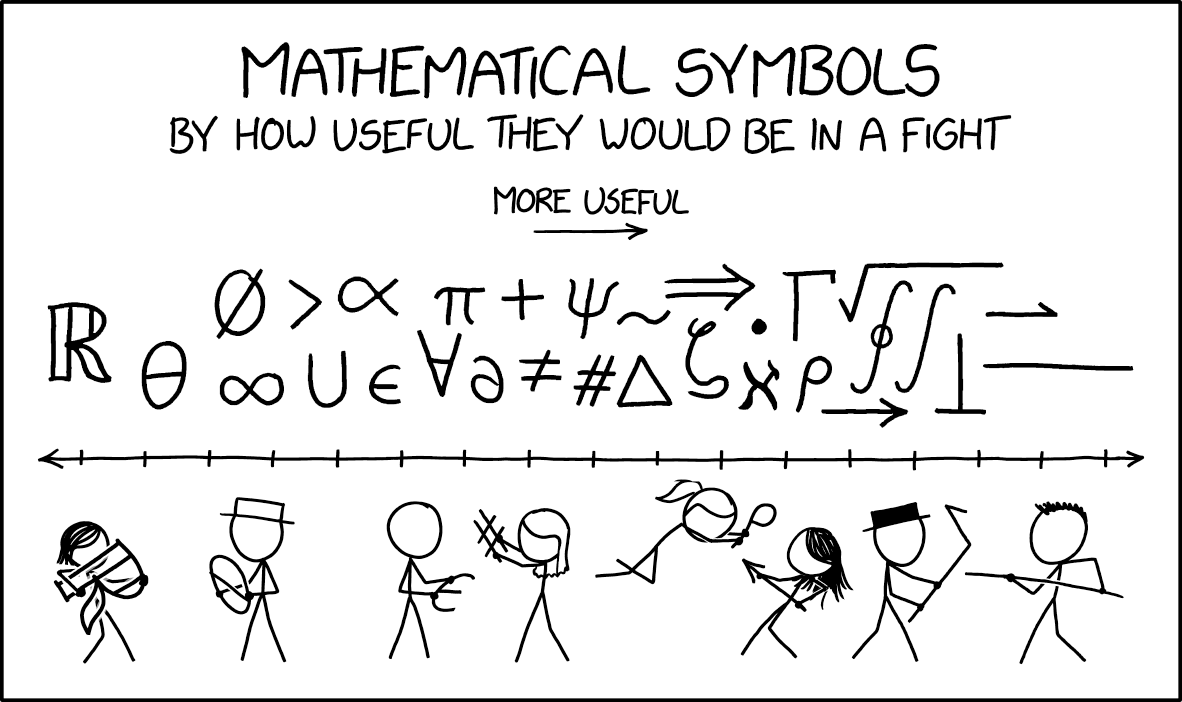
\includegraphics[width=\textwidth]{mathematical_symbol_fight_2x.png} % or tikz or anything
  \end{figure}
% xkcd_2343

As physicists the most important binary relation is none of those things\footnote{I thank Yuval Grossman teaching me this.}. What we usually care about is  $\sim$.\footnote{I use this the same way as $\propto$, which is completely different from `approximately,’ $\approx$.} The symbol $\sim$ tells us how how something \emph{scales}. If I double a quantity on the right-hand side, how does the quantity on the left-hand side scale? Does it depend linearly? Quadratically? Non-linearly? The answer encodes something important about the underlying physics of the system. The symbol $\sim$ the reason why \emph{imagine the cow is a sphere} is a popular punchline in a joke about physicists. 


Implicit in this discussion is the pragmatic policy that we will not care about stray factors of 2 in this class. As my adviser used to say, if you are worried about a factor of 2, then you have addition homework to figure out that factor of 2.\footnote{That being said, you are reading these notes and find an error, do let me know about it.} 

\subsection{Units}

There is another way in which physics is different from mathematics. It is far more prosaic. \emph{Quantities in physics have units}. We do deal in simply numbers, we deal with kilograms, electron volts, meters. It turns out that dimensional analysis is a big part of what we do as physicists. 

\begin{exercise}
Explain, in words, why the quantity $\sin(3~\text{cm})$ is absolute nonsense in any context. What about $\text{exp}(2~\text{kg})$?
\end{exercise}


\section{Converting Units}

Imagine that you have three apples. This is a number (three) and a unit (apple). The meaning of the unit depends on what you're using it to measure. For example, if apples are \$1 each, then you could use an apple as a unit of currency. The way to do this is to simply \emph{multiply by one}:
\begin{align}
  (3\text{ apples}) \times \left(\frac{\text{\$ 1}}{\text{apple}}\right)
  &= \$ 3 \ .
\end{align}
We have used the fact that the exchange rate is simply the statement that
\begin{align}
  1\text{ apple} &= \$1
  & \Rightarrow &&
  1 &= \frac{\$ 1}{1\text{ apple}} \ .
\end{align}
You can do a similar thing for [kilo-]calories or any other conversion rate. 

All that matters is that the conversion factor is a constant. The constants of nature make very good `exchange rates.' For example, high-energy physicists use \textbf{natural units}\index{natural units}:
\begin{align}
  \hbar = c = 1 \ .
\end{align}
At face value, this does not make sense. $\hbar$ has units of action, $c$ is a speed, and 1 is dimensionless. In more conventional units,\footnote{For the most part, we are happy with one significant figure in this course.}
\begin{align}
  c &= 3 \times 10^{10}~\text{cm}/\text{s} 
  &
  \hbar &= 10^{-34}~\text{kg}~\text{m}^2/s
  \ .
\end{align}
However, because nature gives us a \emph{fundamental} unit of action and a \emph{fundamental} unit of speed, we may use them as conversion factors (exchange rates). If $c=1$, then 
\begin{align}
  1~\text{s} &=  3 \times 10^{10}~\text{cm} \ .
\end{align}
This connects a unit of time to a unit of distance. By measuring time, the constant $c$ automatically gives an associated distance. The physical relevance of the distance is tied to the nature of the fundamental constant: one second (or `light-second') is the distance that a photon travels in one second. Observe that this only works because $c$ is a constant. 

\section{Quantifying units}

We use the notation that a physical quantity $Q$ has \textbf{dimension}\index{dimension} $[Q]$ that can be expressed in terms of units of length, mass, and time:
\begin{align}
  [Q] = L^a M^b T^c \ .
\end{align}
The {dimension} is the statement of the powers $a$, $b$, and $c$. You may want to also include units of, say, electric charge. Sticklers may pontificate about whether electric charge formally carries a new unit or not. 


\begin{example}
What are the units of force? We remember that $\vec{F} = m\vec{a}$, so 
\begin{align}
  [\vec F] &= [m][\vec{a}] = M\times L T^{-2} = L^1 M^1 T^{-2} \ .
  \label{eq:02:force:units}
\end{align}
\end{example}

\begin{exercise}
What are the units of the fine structure constant?
\end{exercise}


When working in \textbf{natural units}, $c=1$ means that units of length and time are the same and $\hbar = 1$ means that units of time and energy (mass) are inversely related. In natural units, one simply writes $[Q]$ to mean the mass-dimension of a quantity. To revert back to conventional units, one simply multiplies by appropriate factors of $1=c$ and $1=\hbar$. 

\begin{example}
What are the units of force in natural units? From \eqref{eq:02:force:units} we multiply by one to convert length and time into mass dimensions:
\begin{align}
  [\vec F] &= [c^{-3} \hbar \vec{F}] = M^2 \ .
\end{align}
In natural units we say $[\vec F] = 2$. Recall that energy and mass have the same dimension, which you may recall from the Einstein relation $E^2 = m^2c^4 + p^2c^2$.
\end{example}

\section{Dimensional analysis at work}


\subsection{Sanity Check}

The simplest use of dimensional analysis is to check your work. The following expression is obviously wrong:
\begin{align}
  1 + (3~\text{cm}) \ .
\end{align}
This does not make sense. You cannot sum terms with different dimensions. Similarly, $\sin(3\text{ cm})$ does not make sense. What about $e^{5~\text{cm}}$? This doesn't make sense because
\begin{align}
  e^x = 1 + x + \frac{1}{2!} x^2 +  \cdots
\end{align}
Since each term comes with a different power of $x$, the argument of the exponential must be dimensionless. 

\begin{example}
As pointed out by Matta et al.\footnote{\emph{J.~Chem.~Educ.} 2011, 88, 1, 67–70. \url{https://doi.org/10.1021/ed1000476}}, this argument is not quite correct. Each term in the Taylor expansion of a function $f(x)$ maintains the dimensions of $f(x)$, as is obvious when written out carefully:
\begin{align}
  f(x_0+\Delta x) = f(x_0) + \left.\frac{df}{dx}\right|_{x_0}\Delta x + \frac{1}{2}\left.\frac{d^2f}{dx^2}\right|_{x_0}\Delta x^2 + \cdots \ .
\end{align}
The units of every $dx^2$ in the `denominator' of $d^{(n)}f/dx^n$ is canceled by the units in $\Delta x^n$, no matter what the dimensions of $\Delta x$ are.
%
The real issue is that for many functions, $f(x_0)$ is simply not defined for dimensionful arguments. This is certainly true for trigonometric functions. For the exponential, one may fall back to the limit definition:
\begin{align}
  e^x = \lim_{n\to\infty} \left(1+ \frac{x}{n}\right)^n \ ,
\end{align}
where it is now an issue of different terms having different dimensions. Note that the right-hand side is not a Taylor expansion. The exponential definition above is handy because it makes sense even when $x$ is a matrix or operator.
\end{example}

\begin{exercise}
Sometimes you may think it is useful to keep track of radians (or degrees) as a dimensionful quantity. This, by the way, is a slippery slope because then you may want to think of $\pi$ as some unit of circles... whatever that means. Following the exercise above, show that (1) each term in the Taylor expansion of $f(x) = \sin(x)$ has the same dimensions, and (2) that there is no issue with trigonometric functions being defined as having `dimensionful' arguments in this way.
\end{exercise}

\begin{exercise}
Consider the energy spectrum of light emitted from some constant source---a distant star, the ongoing annihilation of dark matter in the galactic center, or a high-intensity laser. The spectrum encodes how many photons are emitted per unit time. We can plot this spectrum as a curve on a graph. We can even normalize the curve so that it integrates to one photon. This means we only care about the distribution of energy, not the absolute amount. The horizontal axis of such a plot is the photon energy. What are the units of the vertical axis?
\end{exercise}

\subsection{Solving problems}

Here is a common problem in introductory physics. Assume you have a pendulum with some sufficiently small initial displacement $\theta_0$. What’s the period, $\tau$ of the pendulum? We draw a picture like Fig~\ref{fig:simple_pendulum}.
%
% \marginfig{figures/lec01_pendulum.pdf}{Sketch of a simple pendulum.}{fig:simple_pendulum}
\begin{figure}[tb]
	\centering
	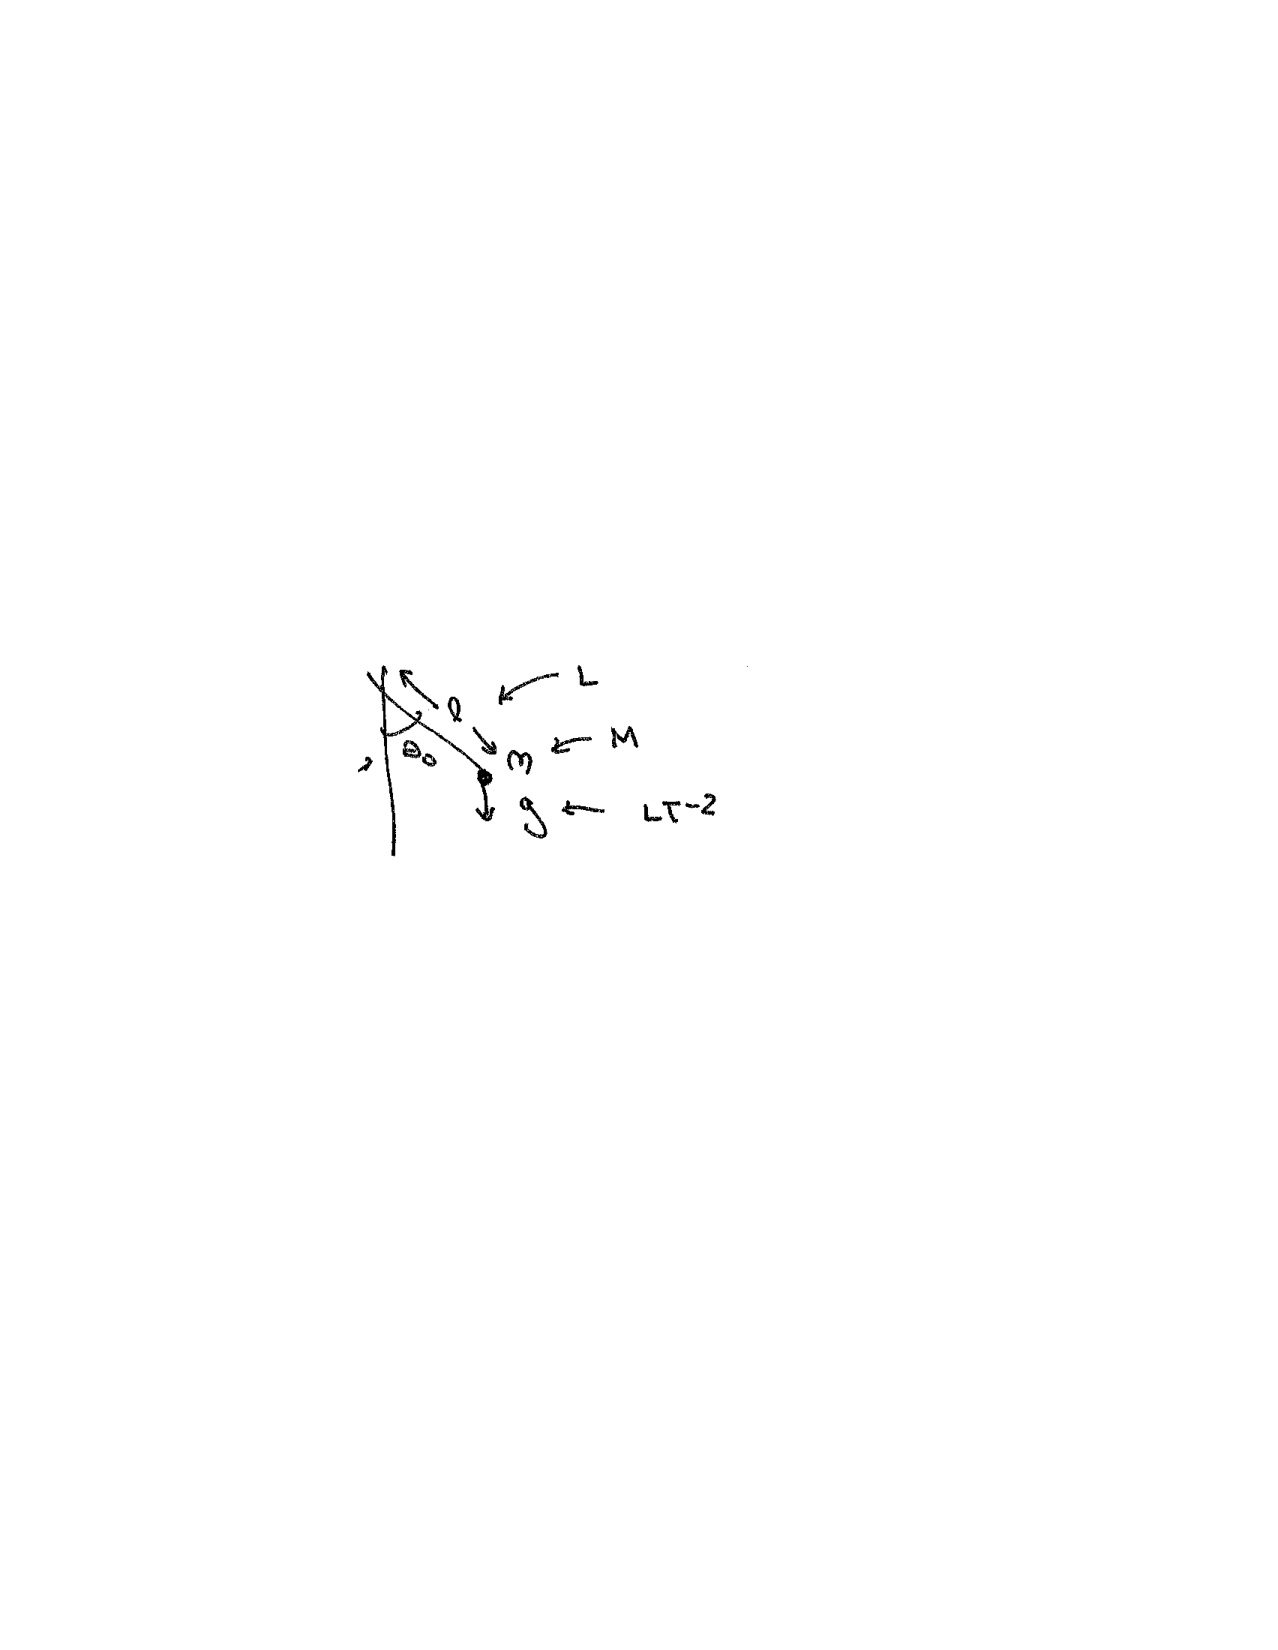
\includegraphics[width=.5\textwidth]{figures/lec01_pendulum.pdf}
	\caption{Sketch of a simple pendulum.}
	\label{fig:simple_pendulum}
\end{figure}
%
%
From dimensional analysis, we know that the period has dimensions of time, $[\tau] = T$. The problem gives us a length $[\ell]=L$ and the gravitational acceleration, $[g]=LT^{-2}$. Note that $[\theta_0] = 1$ is dimensionless. This means that the only way to form a quantity with dimensions of time is to use $g^{-1/2}$. This leaves us with a leftover $L^{-1/2}$, which we can fix by inserting a square root of $\ell$:
\begin{align}
  \tau \sim g^{-1/2} \ell^{1/2} \ .
\end{align}
If we want to be fancy, we can make this an equal sign by writing a function of the other dimensionless quantities in the problem:
\begin{align}
  \tau = f(\theta_0) \sqrt{\frac{\ell}{g}} \ .
\end{align}

\flip{To do: include problems from R.W.~Robinett \emph{American Journal of Physics} \textbf{8}3, 353 (2015); \url{https://doi.org/10.1119/1.4902882}.}


\subsection{Scaling}

A key theme in physics is scaling relations. We present a somewhat contrived example of how this works adapted from section 11 of V.\ I.\ Arnold's \emph{Mathematical Methods of Classical Mechanics}.\footnote{This is one of my favorite differential geometry textbooks because it is disguised as a book on mechanics.}. Suppose you have some static, central potential $U(\vec r)$. Maybe it’s some planet orbiting a star. 
%
% \textfig[1]{figures/lec01_orbit.pdf}{A orbital trajectory, $\vec{r}_0(t)$.}{fig:simple_orbit}
\begin{figure}[tb]
	\centering
	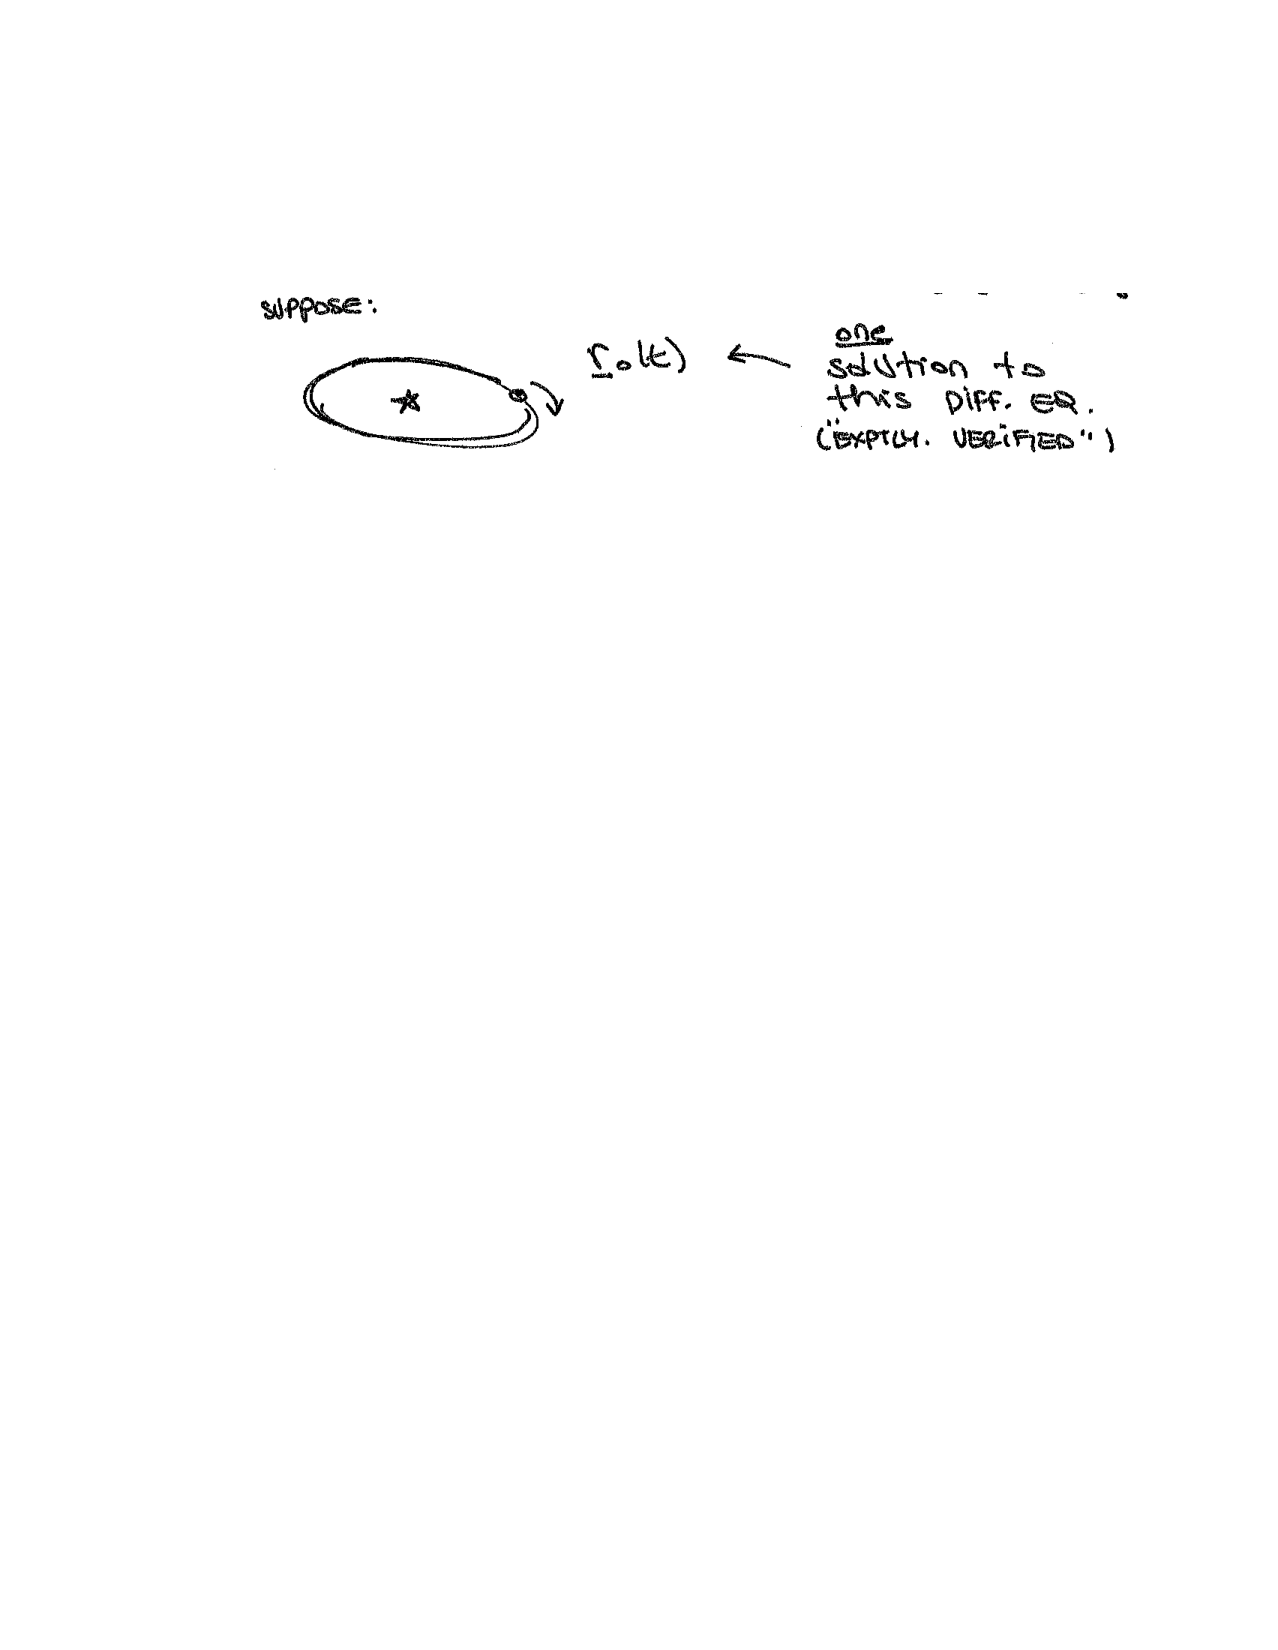
\includegraphics[width=.5\textwidth]{figures/lec01_orbit.pdf}
	\caption{A orbital trajectory, $\vec{r}_0(t)$.}
	\label{fig:simple_orbit}
\end{figure}
%
The force law gives:
\begin{align}
  m 
  \ddot{\vec{r}} = - \frac{\partial U}{\partial\vec{r}} \ .
  \label{eq:scaling:eg}
\end{align}
Suppose we are given a solution, $\vec r_0(t)$. Perhaps this is a trajectory that is experimentally verified. Dimensional analysis gives us a way to scale this solution into other solutions. For example, let us scale time by defining a new variable $t'$:
\begin{align}
  t \equiv \alpha t' \ .
\end{align}
Because the potential is static, then only the left-hand side of the force law changes. Even though the right-hand side formally has dimensions of time, $T^{-2}$, it does not transform because those units are carried in a constant, perhaps $G_N$, not a $(d/dt)^2$ like the left-hand side. The left-hand side of the force law gives:
\begin{align}
  m\left(\frac{d}{dt}\right)^2 \vec r_0(t) 
  &=
  m\alpha^{-2} \left(\frac{d}{dt'}\right)^2 \vec r_0(\alpha t') \ .
\end{align}
This begs us to define a new mass $m' = m\alpha^{-2}$ so that
\begin{align}
   m' \left(\frac{d}{dt'}\right)^2 {\vec{r}_0}(\alpha t')
  = - \frac{\partial U}{\partial\vec{r}_0} \ .
\end{align}
What this tells us is that we may define a new trajectory, $\vec r_1(t') \equiv \vec{r}_0(\alpha t')$, which is a solution in the same potential that traces the same trajectory but at $\alpha$ times the speed and with mass $m'$. Changing labels $t'\to t$ for a direct comparison:
\begin{align}
   m' \left(\frac{d}{dt}\right)^2 {\vec{r}_1}(t)
  = - \frac{\partial U}{\partial\vec{r}_1} \ ,
\end{align}
which is indeed\footnote{We were able to swap $\vec r_0$ with $\vec r_1$ simply because $U$ only depends on the position.} \eqref{eq:scaling:eg} with a new mass $m'$ and a trajectory $\vec r_1(t') \equiv \vec{r}_0(\alpha t')$. For example, if $\alpha = 2$, then $\vec r_1(t)$ traces the same trajectory at double the velocity with one fourth of the mass.

\begin{exercise} 
I missed something in the example above. In order for a planet of mass $m'$ to have trajectory $\vec r_1(t')$, what is the mass of the star compared to the original mass $M_\star$?\footnote{Thanks to Eric Zhang (2021) for pointing this out.} 
\end{exercise}

\begin{example} 
Business-y people like to quantify effort using words like `person--hour' or `person--years.' This is the idea that a 10 person--hour task would take 10 people one hour to complete, or one person 10 hours to complete, or 5 people two hours to complete, etc.  As you can see, this choice of units implies that effort has a linear scaling in both the number of people and the amount of time needed. Anyone who has worked on a group project knows that this linear scaling is bullshit. Frederick Brooks reflects on this in the 1974 essay, ``Myth of the Man--Month.''\cite{Brooks1975}
\end{example}

\subsection{Error Estimates}

This section is based on a lovely \emph{American Journal of Physics} article by Craig Bohren.~\cite{doi:10.1119/1.1574042}%\footnote{\url{https://doi.org/10.1119/1.1574042}} 
Let us go back to another high school physics problem: we drop a ball of mass $m$ from height $h$. See Fig.~\ref{fig:simple_drop}. The task is to find the time $t_0$ for the ball to hit the ground.
%
% \marginfig{figures/lec01_drop.pdf}{Dropping a ball of mass $m$.}{fig:simple_drop}
\begin{figure}[tb]
	\centering
	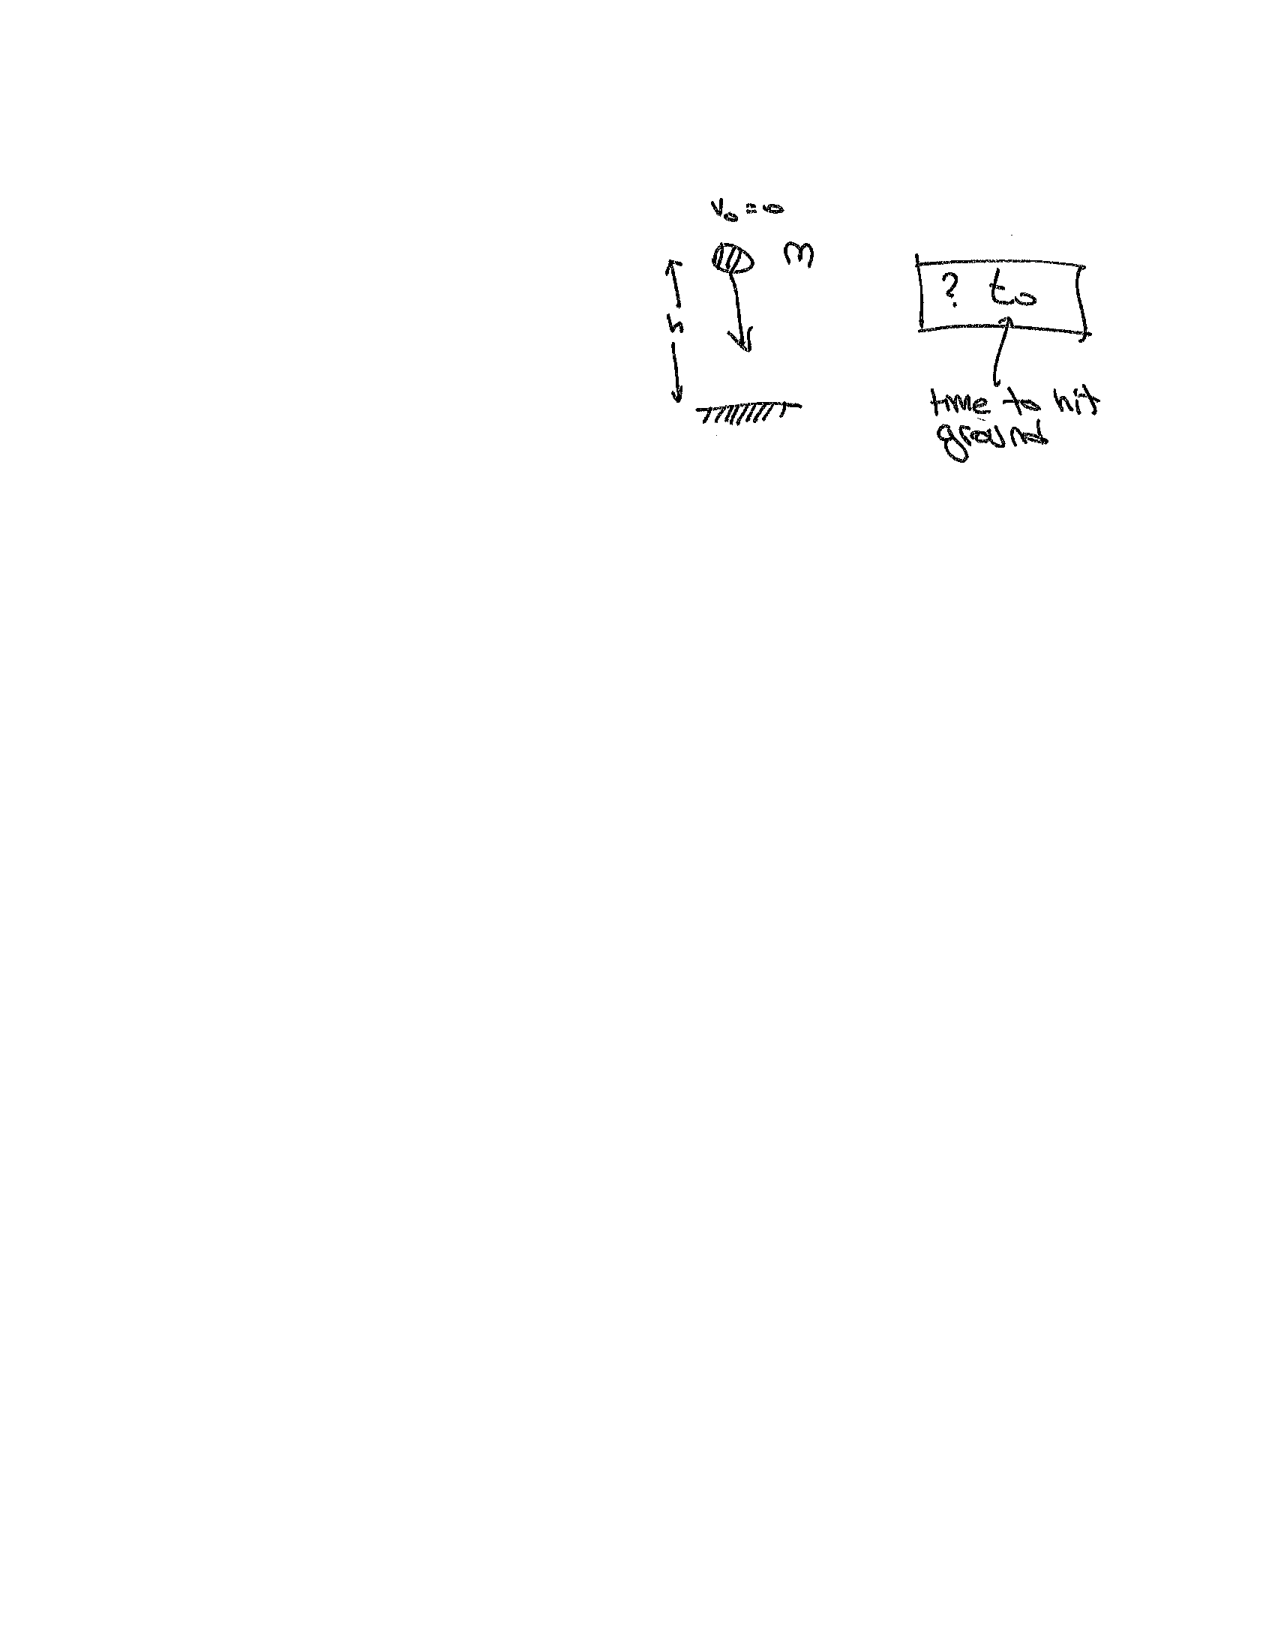
\includegraphics[width=.5\textwidth]{figures/lec01_drop.pdf}
	\caption{Dropping a ball of mass $m$.}
	\label{fig:simple_drop}
\end{figure}

% Suppose you drop a mass $m$ from height $h$ that is initially at rest. How long before this hits the ground? 
You can integrate the force equation to get
\begin{align}
  t_0 = \sqrt{\frac{2h}{g}} \ .
\end{align}
This is the \emph{exact} answer \emph{within our model} of the system. The model made several assumptions: the mass is a point mass, the gravitational acceleration is constant at all positions, there is no air resistance, etc. In fact, we \emph{know} that if we do an experiment, our result will almost certainly \emph{not} be $t_0$. All we know is that $t_0$ is probably a good approximation of the actual answer. What we would like to to know is: \emph{how good of an approximation is it?}

One way to check this is to do the next-to-leading order (\acro{NLO}) calculation, taking into account a more realistic model and then compare to $t_0$. Of course, ``more realistic'' is also code for ``more complicated.'' Take a moment to appreciate that doing this is \emph{stupid}. Why do we need to do a \emph{hard} calculation to justify doing an \emph{easy} one? If we are going to do the hard calculation anyway, what was the point of ever doing the easy one?

What we really want is an error \emph{estimate}. The error\index{error} is
\begin{align}
  \epsilon &= \frac{t_1 - t_0}{t_0} \ .
\end{align}
This is a dimensionless quantity that determines how far off $t_0$ is from a more realistic calculation, $t_1$. Ideally we should not actually have to do much work to estimate $t_1$. 

Let us assume that we are not completely nuts and that we are in a regime where the error is small\footnote{Note the error has to be dimensionless in order for us to be able to call it `small,` otherwise it begs the question of `small with respect to what?'}. Then the error is a function of some dimensionless parameters, $\xi$, in the system. We define these $\xi$ so that as $\xi \to 0$, $\epsilon(\xi) \to 0$. In other words, the approximation gets better as the $\xi$ are made smaller. By Taylor expansion:
\begin{align}
  \epsilon(\xi) = \epsilon(0) + \epsilon'(0) \xi + \mathcal O(\xi^2) \ .
\end{align}
By assumption, $\epsilon(0) = 0$ and $\mathcal O(\xi^2)$ is  small. We can then make a reasonable \emph{assumption} that the dimensionless value $\epsilon'(0)$  is $\mathcal O(1)$. This tells us that the error goes like $\epsilon(\xi) \sim \xi$.

By the way $\mathcal O(1)$ is read ``order one'' and is fancy notation for the order of magnitude. Numbers like 0.6, 2, and $\pi$ are all $\mathcal O(1)$. A number like $4\pi$, on the other hand, is $\mathcal O(10)$.  The assumption that a dimensionless number is $\mathcal O(1)$ is reasonable. When nature gives you a dimensionless parameter that is both (a) important and (b) very different from $\mathcal O(1)$, then there's a good chance that it's trying to tell you something about your model. Good examples of this are the cosmological constant, the strong \acro{CP} phase, and the electroweak hierarchy problem.\footnote{There are also `bad' examples. The ratio of the angular size of the moon to the angular size of the sun is unity to very good approximation. This is quite certainly a coincidence. Our universe appears to be in an epoch where the density of matter, radiation, and dark energy all happen to be in the same ballpark. Our cosmological models imply that this is purely a coincidence. It would be very curious if this were not the case. As an exercise, you can critically explore the use of the anthropic principle in physics.} 

Here is how it works in practice. One effect that we miss in our toy calculation of $t_0$ is that the earth is round with radius $R$. This means that assuming a constant $g$ is an approximation. We have two choices for a dimensionless parameter $\xi$:
\begin{align}
  \xi &= \frac{h}{R}
  &\text{or}&&
  \xi &= \frac{R}{h} \ .
\end{align}
There is an obvious choice: $\xi = h/R$, because we know that as $h$ is made smaller (drop the ball closer to the ground) or $R$ becomes bigger (larger radius of Earth) then the constant $g$ approximation gets better. We thus expect that the corrections from the position-dependence of $g$ go like $\mathcal O(h/R)$.
 
% Exercise: check by explicit calculation, 2017 lec 1
\begin{exercise}
Check by explicit calculation that the correction to the constant $g$ approximation is linear in $h/R$. Start by writing the force law for a point source of at distance $r=R+h$ from the center of the Earth. Taylor expand to find a second order differential equation that is difficult to solve:
\begin{align} 
  \ddot{h} = \frac{-g}{\left(1+\frac{h}{R}\right)^2} \ .
\end{align}
Taylor expand to reduce this to an equation of the form
\begin{align}
  \frac{d^2 q}{ds^2} = -1 + 2q \ ,
\end{align}
Here we define the natural dimensionless variables, $q = h/R$ and $s = \left(g/R\right)^{1/2} t$. If the choice of $s$ is not obvious, please do everything in terms of $t$ and then observe that one can conveniently absorb a factor of $g/R$ into dimensionless time variables.\footnote{You should find an equation of the form $\ddot q = -(g/R)(1-\cdots)$.} Plug the dimensionless differential equation into \emph{Mathematica} or your favorite symbolic solver to obtain 
\begin{align}
  q(s) = c_1 e^{\sqrt{2}s} + c_2 e^{-\sqrt{2} s} + \frac{1}{2} \ .
\end{align}
Argue that the initial condition $\left.\dot h(t)\right|_{t=2} = 0$ implies that the coefficients satisfy $c_1 = c_2$ so that you can combine the exponentials into a hyperbolic cosine. 
% If $q_0$ is the value of $q(s)$ at $t=0$, show that $c_1 = (q_0  - 1/2)/2$.
Show that one obtains:
\begin{align}
  \frac{2q(s) - 1}{2q(0) -1} = \cosh(\sqrt{2}s) \ .
\end{align}
Argue why you can Taylor expand the right-hand side about small argument; that is, explain why $s \ll 1$. (Hint: use $h\ll R$.) Perform the Taylor expansion of the hyperbolic cosine to find that the leading correction to the fall time is
\begin{align}
  s_1 = \frac{2q_0}{1-2q_0} \ .
\end{align}
The zeroth order approximation was $s_0 = (g/R)^{1/2} t_0 = \sqrt{2q_0}$. Calculate $(s_1 - s_0)/s_0$ to confirm that this is $\mathcal O(h/R)$. 
\end{exercise}

\subsection{Bonus: Allometry}

There is a fun topic called \textbf{allometry}.\index{allometry} This is basically dimensional analysis applied to biology. A typical example is to consider two people who have roughly the same shape but different characteristic lengths, $\ell$ and $L$, Fig.~\ref{fig:lec1_allometry}.
% \marginfig{figures/lec01_allometry.pdf}{Two mathematically similar people.}{fig:lec1_allometry}
\begin{figure}[tb]
	\centering
	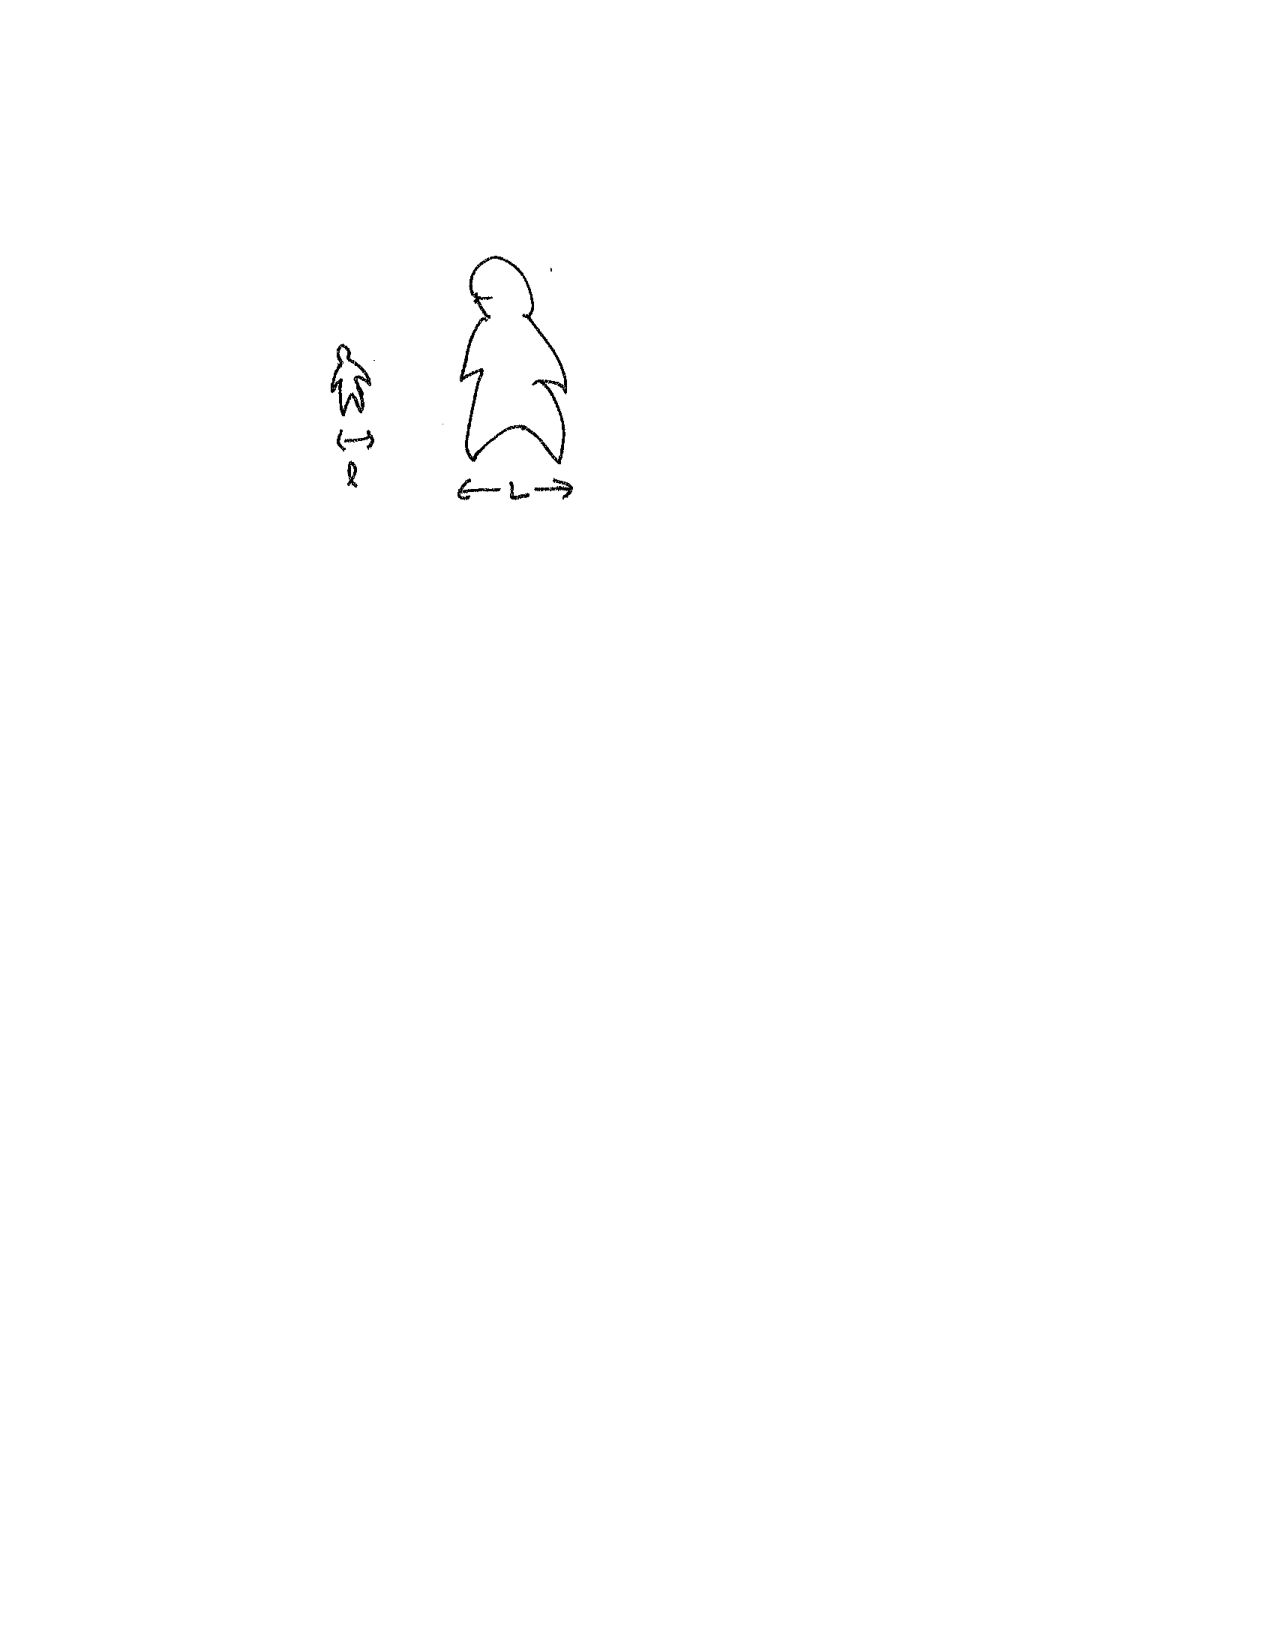
\includegraphics[width=.5\textwidth]{figures/lec01_allometry.pdf}
	\caption{Two mathematically similar people.}
	\label{fig:lec1_allometry}
\end{figure}

% \begin{center}
% 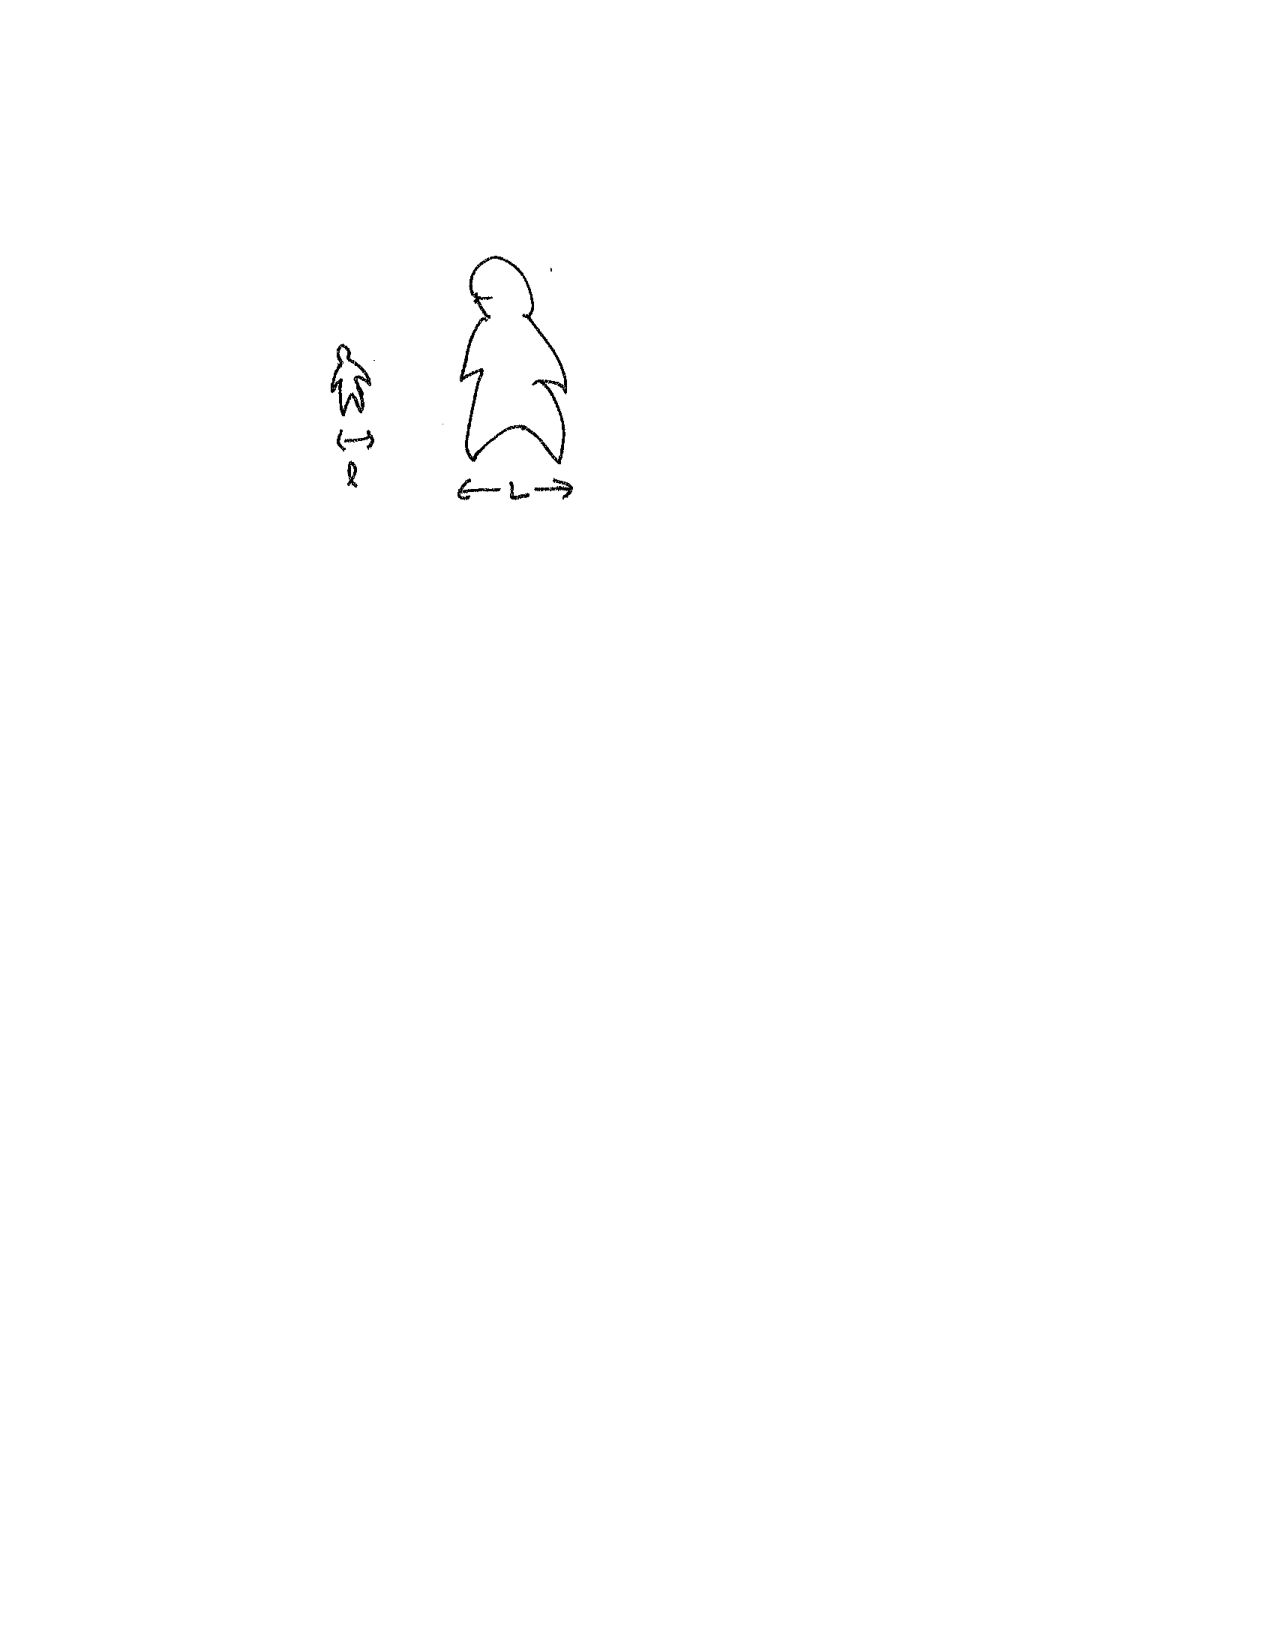
\includegraphics[width=.4\textwidth]{figures/lec01_allometry.pdf}
% \end{center}

\begin{exercise}
If both people exercised at the same rate, which one loses more absolute weight? By how much? Let us assume that weight loss is primarily from the conversion of organic molecules into carbon dioxide. 
\end{exercise}

\begin{exercise}
David Hu won his first IgNobel prize for determining that mammals take about 21 seconds to urinate, largely independently of their size\footnote{I learned about this in his excellent popular science book, \emph{How To Walk on Water and Climb Up Walls}.}. Can you use dimensional analysis to argue why this would be the case? It may be helpful to refer to the paper\cite{doi:10.1073/pnas.1402289111}. As you read it, figure out which terms are negligible (and in what limits), identify the assumptions of the mathematical model (scaling of the bladder and urethra), and prove the approximate scaling relation. Make a note to yourself of which steps were non-trivial and where one may have naively mis-modeled the system. By the way, David Hu won a second IgNobel prize for understanding wombats' cubical poop.
\end{exercise}

The above exercise on mammalian urination is a good example of \emph{modeling}.\index{model} As physicists, we must identify and make a mathematical model for the most salient features of a problem. We must also be able to quantify the error from neglecting sub-leading contributions. As a rough model for scaling purposes, we can ignore viscosity and surface tension effects on human-sized mammals. For much smaller mammals, these effects become larger---the authors of the study note that mice tend to urinate droplets---in which case one can ignore the `inertial' $\frac{1}{2} \rho v^2$ term in Bernoulli's equation. For human-sized mammals, we may assume that steady state urination is given by Bernoulli's equation:
\begin{align}
  P + \rho g h = \frac{1}{2}\rho v^2 \ ,
\end{align}
where $P$ is the pressure from the bladder, $h$ is the column height of the urethra, $\rho$ is the mass density of urine, and $v$ is the velocity of the urine at the end of the urethra. Let us simplify to the condition where urination is purely driven by gravity---that is, the bladder does not exert any additional pressure, $P=0$. You can now show that the total urination time scales like the mass of the mammal to the one-sixth power, $\tau \sim M^{1/6}$. That is, the urination time has a very weak scaling dependence on how massive the mammal is.

\begin{exercise}
In August 2021, Ezra Klein interviewed Dr.~C\'eline Goudner about the \acro{COVID-19} variant.~\cite{klein_2021} In the interview, Klein cited the statement that the Delta variant has $\mathcal O(1000)$ times the viral load than prior \acro{COVID} strains. Goudner then interprets this in the following way: if the \acro{CDC} defined `close contact' for prior strains as 15 minutes of being indoors with an infected invdividual without a mask, then the equivalent `close contact' time for the Delta variant is around \emph{one second}. What scaling assumptions go into that estimate? Some of these assumptions are not obvious to me: for example, parts of the respiratory have a fractal-like structure that would lead me to suspect fractal scaling dimensions for surface area. \acro{Remark}: Just because you know dimensional analysis, that does not make you a medical, healthcare, or public policy expert.\footnote{Early in the \acro{COVID-19} pandemic, many physicists became armchair  modelers of epidemics. Some of this was driven by hubris about our mathematical intuition. Many of the physicists lost interest when their models aligned poorly with what actually happened.} 
\end{exercise}

The following exercises draw from an article by Nicole Meyer-Verneta and Jean-Pierre Rospars in the American Journal of Physics\cite{doi:10.1119/1.4917310} and the references therein.
 \begin{exercise}
 Estimate the expected velocity of an All Terrain Armored Transport (\acro{AT}-\acro{AT})\footnote{\url{https://starwars.fandom.com/wiki/All_Terrain_Armored_Transport}} of characteristic height $L$. You can assume that the walking behavior is based on a pendulum. \acro{Answer}: $v \sim \sqrt{Lg}/2\pi$.
 \end{exercise}

 \begin{exercise}
 Based on the density $\rho$, the force-per-cross-sectional area $\sigma$, and the maximum rate of energy consumption per unit mass $b$, one may estimate the `sprint' velocity of an animal of length $L$. This sprint velocity is conveniently described with respect to the dimensionless `body lengths per time,' $v_\text{spr}/L$.

Remarkably, for over 20 orders of magnitude in animal length $L$, the value of $v_\text{spr}/L$ is within an order of magnitude of 10/sec:
\begin{center}
 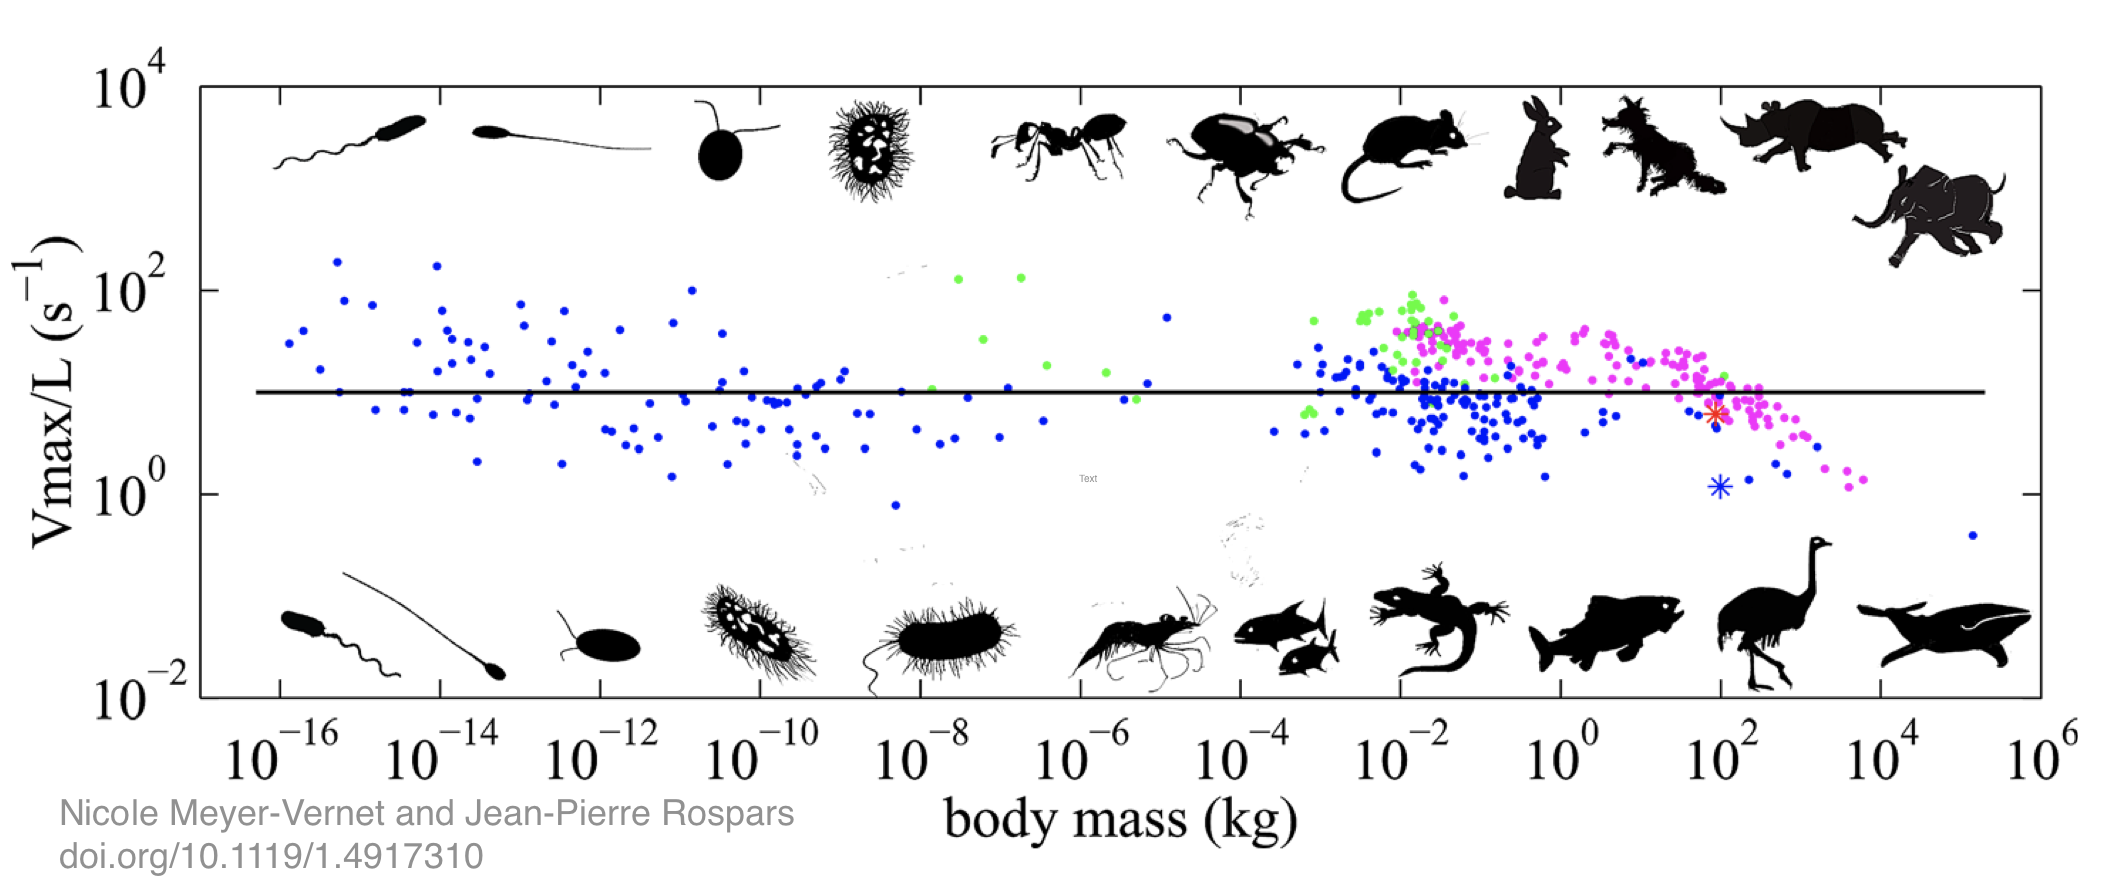
\includegraphics[width=.\textwidth]{figures/allometry_meyer-verneta.png}
\end{center}
% \textfig[1]{figures/allometry_meyer-verneta.png}{Image from Meyer-Verneta and Rospars.~\cite{doi:10.1119/1.4917310}}{fig:allometry_meyer-verneta}


Argue from dimensional analysis that $v_\text{spr}/L \sim b\rho/\sigma$. (This is the easy part.) It turns out that there are simple physical principles for each of these terms to be roughly constant for all life on Earth (this is the more subtle part); see the article for a discussion.
\end{exercise}

\begin{exercise}
The height of trees. How does the maximum height of a tree, $L$ scale with the diameter of its cross section, $d$? For an argument that $L\sim d^{3/2}$, see Thomas McMahon's article ``The Mechanical Design of Trees'' in \emph{Scientific American} volume 233 (1975)\footnote{\url{https://www.jstor.org/stable/24949846}}. McMahon was the first to propose a physical explanation for the observed scaling law that the metabolic rate of an animal scales like the characteristic size to the 3/4 power. A nice bibliography of his work can be found in \emph{Annual Review of Biomedical Engineering}.~\cite{doi:10.1146/annurev.bioeng.3.1.0}
\end{exercise}